\section{Ejercicio 2}

\subsection{Introducción}
Este ejercicio consiste en entrenar una red neuronal que aprenda a predecir los valores de calor y refrigeración para un edificio, dado un set de datos
con características de cada edificio. A diferencia del Ejercicio 1, se deberá entrenar un modelo de regresión ya que la red tiene que devolver valores
numéricos y no clases.

\subsection{Experimentación}
Para los siguientes experimentos se utilizo una arquitectura de red con la siguiente topología: 8 entradas, 1 capa oculta de 16 unidades y 2 unidades de salida,
tal como se muestra en la figura a continuación.

\begin{figure}[H]
  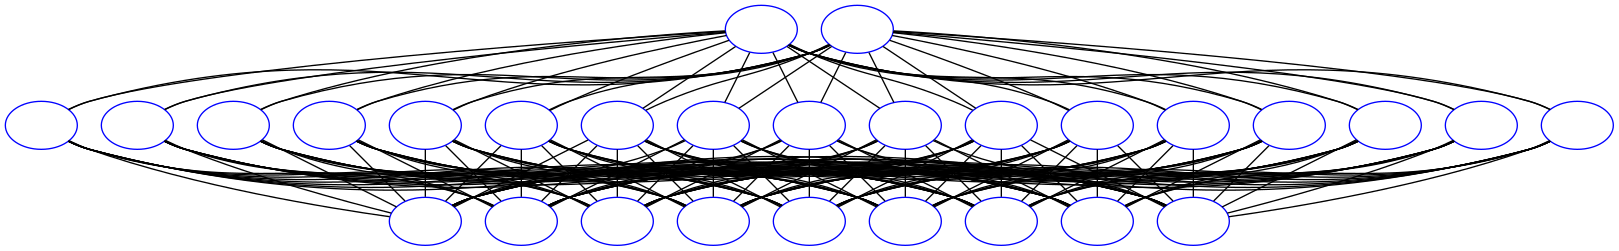
\includegraphics[width=12cm, height=5cm]{../plot/9-17-2.png}
  \centering
  \caption{Red utilizada (9-17-2)}
\end{figure}

Cabe mencionar que para todos los experimentos se utilizo un $\eta$ = 0.02, 500 épocas de entrenamiento y un modo de entrenamiento estocástico.
\subsubsection{Experimento 1}
Para este experimento se decidió evaluar el efecto de preprocesar tanto los valores de entrada como de salida de la red propuesta a fin de observar su
comportamiento. Se utilizaron funciones de activación sigmoidea para la primer capa y lineal para la salida (debido a que la salida debe estar entre 0 y 50 aproximadamente,
 sin normalizar la salida). El preprocesado consistió en restarle a cada muestra la media y luego dividirlo por la varianza, es decir que por cada valor de la entrada
como de salida se lo reemplazo por la siguiente formula:
\begin{equation}
  \dot{x_{i}} = (x_{i} - \mu_{input}) / \sigma_{input}
\end{equation}

\begin{equation}
  \dot{y_{i}} = (y_{i} - \mu_{output}) / \sigma_{output}
\end{equation}

Los resultados obtenidos se presentan a continuación:

\begin{figure}[H]
  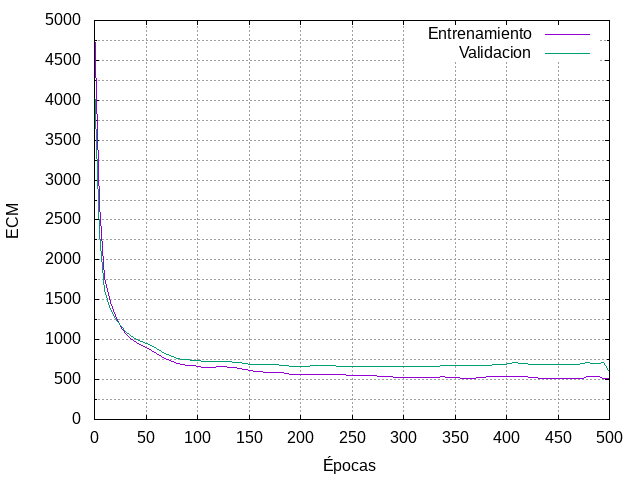
\includegraphics[width=125mm]{imagenes/ej2/ex_1-1_red-9-17-2_errors.png}
  \caption{Con preprocesamiento de entrada}
\end{figure}

\begin{figure}[H]
  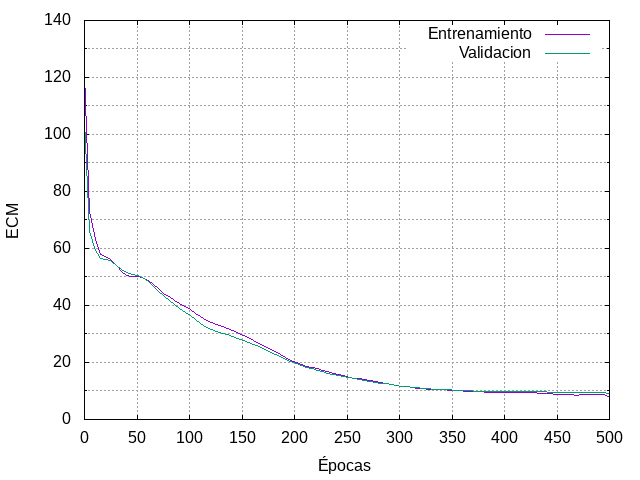
\includegraphics[width=125mm]{imagenes/ej2/ex_1-2_red-9-17-2_errors.png}
  \caption{Con preprocesamiento de entrada y de salida}
\end{figure}

Se observó una amplia diferencia entre ambos entrenamientos ya que el ECM es mucho menor en el caso en que se preprocesa la salida, llegando
a mínimos muy diferentes. Con este experimento se evidencia la importancia del pre procesamiento de los datos de entrenamiento.

Debido al peso de estos resultados se decidió seguir entrenando sobre la misma red y preprocesando la salida.

\subsubsection{Experimento 2}
Este experimento consistió en variar las funciones de activación de la capa oculta. Se decidieron utilizar funciones de tipo \textit{Tangente hiperbólica} y \textit{ReLu}
para analizar comportamientos y performance de la red. Los resultados que se obtuvieron fueron los siguientes:

\begin{figure}[H]
  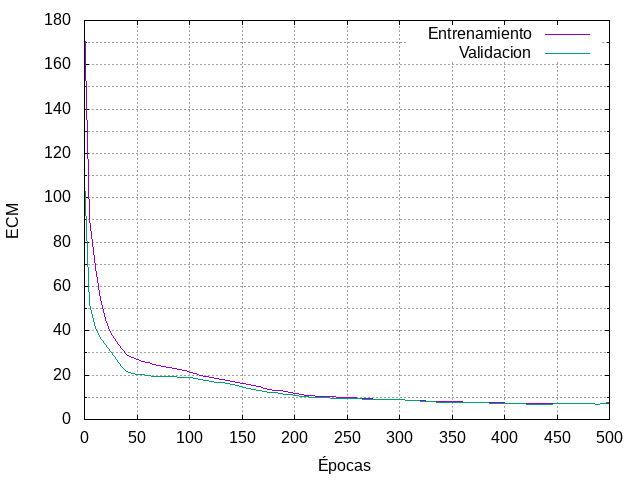
\includegraphics[width=125mm]{imagenes/ej2/ex_2-1_red-9-17-2_errors.png}
  \caption{Función de activación Tangente Hiperbolica}
\end{figure}

\begin{figure}[H]
  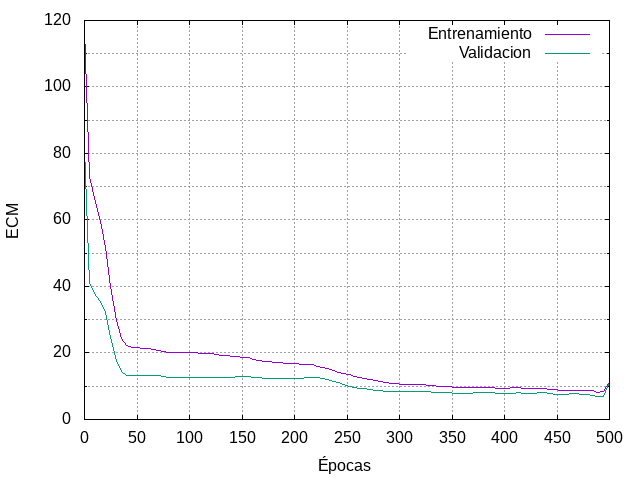
\includegraphics[width=125mm]{imagenes/ej2/ex_2-2_red-9-17-2_errors.png}
  \caption{Función de activación ReLu}
\end{figure}

Se observó que los resultados son bastantes similares, dado que ambas funciones de activación se compartan parecido. Sin embargo, la Tangente hiperbólica tiene un poco menos
de ECM que la ReLu, es por esto que se decidió continuar utilizando la función de activación de Tangente hiperbólica para la experimentación restante.

\subsubsection{Experimento 3}
Para este experimento se decidió variar la función aleatoria de generación de pesos de la red. Se utilizó una distribución uniforme en el rango (-D, D), donde:
\begin{equation}
  D = \frac{1}{\sqrt{i + o}} \mbox{con i= cantidad de entradas de la capa y o = cantidad de salidas de la capa}
\end{equation}

\begin{figure}[H]
  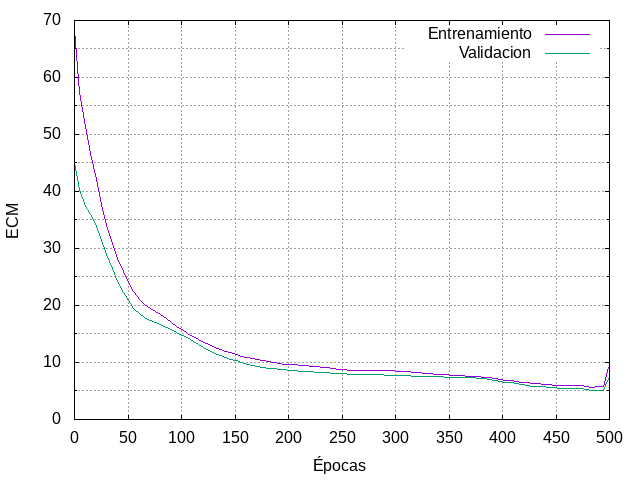
\includegraphics[width=125mm]{imagenes/ej2/ex_3-1_red-9-17-2_errors.png}
  \caption{Con distribución uniforme y función de activación tangente hiperbolica}
\end{figure}

\begin{figure}[H]
  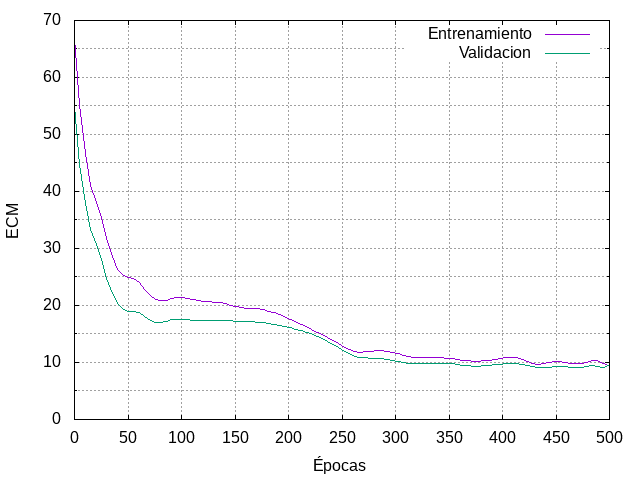
\includegraphics[width=125mm]{imagenes/ej2/ex_3-2_red-9-17-2_errors.png}
  \caption{Con distribución uniforme y función de activación ReLu}
\end{figure}
\subsection{Conclusión}
Pudimos observar que luego de este proceso sobre la base de Test al evaluar la mejor red se obtuvo un error cuadrático medio de 1.44 lo cual es bastante bueno y 
confirma que no se sobreajustaron los parámetros a un set de validación particular.

Una conclusión que se obtuvo luego de experimentar con este ejercicio fue que los problemas de clasificación son mas difíciles de aprender que los de regresión, ya que
los errores obtuvimos en el ejercicio 2 fueron mucho menores a los obtenidos en el ejercicio 1, sin aplicar mejoras al Backpropagation y en una menor cantidad de épocas. \\
Otro punto destacado es la importancia que tiene el hecho de normalizar tanto la entrada como la salida en los ejercicio de regresión, ya que esto lleva a una mejora importante
en la minimización del error obtenido.

Por otra parte se concluyo que la función de activación Relu resuelve los problemas que tienen la funciones tangente hiperbólica y logística al momento de correr el Backpropagation,
en el que si la derivada se encuentra saturada se obtienen valores muy chicos y esto conlleva a errores numéricos en caso de que la entrada no este normalizada \footnote{Este fenómeno es llamado Vanishing gradient problem}. Este fue un problema
que se encontró al experimentar con el trabajo, pero se observó que al normalizar la entrada dejo de ocurrir. 
